

\section{Strategies for using fewer points}

    \begin{itemize}
        \item With general convex constraints, sufficiently poised sets within the feasible region may not exist.
        \item To illustrate, consider finding a fully quadratic model in 2-dimensions.
        \item As the constraints become more thin,
            \begin{itemize}
                \item The model becomes less poised
                \item There is less need for requiring the model to be quadratic in $y$.
            \end{itemize}
        \item We would prefer to use a subset of all quadratics, with fewer points to approximate them.
    \end{itemize}

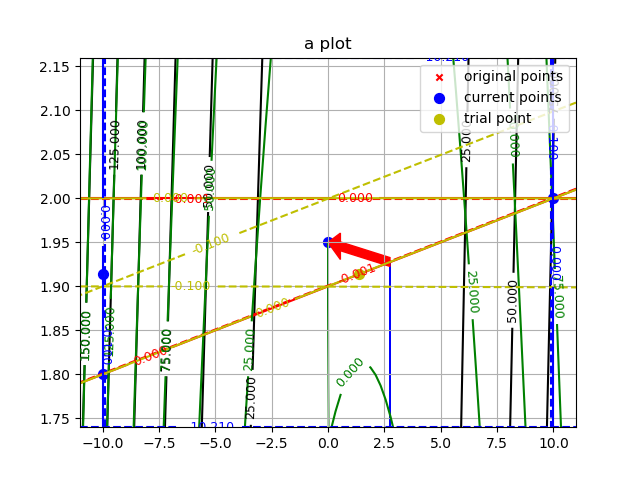
\includegraphics[width=150px]{images/2_2_4_68.png}
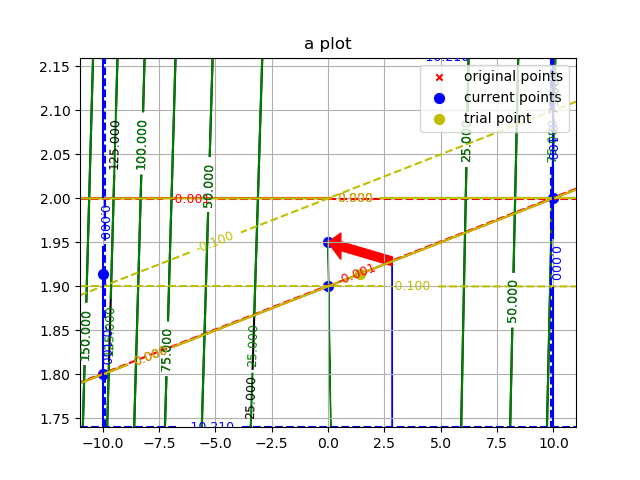
\includegraphics[width=150px]{images/2_3_5_1.png}


\section{Full pivoting}
\begin{itemize}
    \item One approach is to use full pivoting within the LU factorization used compute the Lagrange polynomials.

    \item When there are no more pivots greater than a threshold, the LU factorization terminates, and only uses the points and polynomials already computed after zeroing the remaining entries.
        
    \item This method will provide the next point to use as well as the next polynomial to include.
        
\end{itemize}

\section{Undetermined Coefficients}

